\documentclass{article}
\usepackage[utf8]{inputenc}
\usepackage[english]{babel}
\usepackage{csquotes}

\usepackage{graphicx}               % image packages
\graphicspath{ {images/} }
\usepackage{float}
\usepackage{wrapfig}
\usepackage[rightcaption]{sidecap}

\usepackage[
backend=biber,
style=alphabetic,
citestyle=authoryear-comp 
]{biblatex}
 
\addbibresource{cs4099_bib.bib}     %imports bib file

\usepackage{hyperref}
\hypersetup{
    colorlinks,
    citecolor=black,
    filecolor=black,
    linkcolor=black,
    urlcolor=black
}

\title{CS4099: An Analysis of the Mechanisms and Techniques used in web-based Targeted Advertising}
\author{12001995}
\date{Academic Year 2015-2016}

\begin{document}

\maketitle

\begin{figure}[H]
  \centering
    
\includegraphics[width=0.8\textwidth]{university_logo.png}
\end{figure}

\pagebreak

\tableofcontents

\pagebreak

\section{Abstract}
The innovation of the world wide web has spawned  completely new forms of marketing and advertising. The most prevalent and insidious of these  is targeted advertising. The contemporary network of entities that interact to profile and track individuals and  bid for and place adverts within a website in real time is complex and lacks transparency. This project will  delve into the mechanisms and techniques used by organisations to i) profile individuals; ii) identify them when they are web browsing; iii) create and display targeted adverts to users in real time. It will also i) evaluate methodologies and tools designed to reduce the effectiveness of such advertising; ii) independently validate the background traffic associated with tracking; iii) create a framework of tools and methods to help improve the transparency of web tracking and profiling to the end user; iv) investigate the possibility for detecting digital advertising fraud through an app or plug-in.  


\section{Introduction}
There are numerous techniques used by advertising organisations to gain personal information of users for the purpose of targeted advertising, this paper will look to explore the various techniques and discuss how a user can increase their online privacy.The proceeding sections will present a number of the ways advertisers collect user data and how they are used.  

\section{Targeted Advertising}
Online advertising is an increasingly broad category which takes up a large percentage of advertising budgets worldwide the forecasts of Satistia (2013) state that digital advertising increased to about 121 billion dollars in 2013 and is expected to double by 2018. The Federal Trade Commission (FTC) defines targeted advertising as ``the practice of tracking an individual’s online activities in order to deliver advertising tailored to the individual’s interests'' \parencite{comission2009}. Previous studies have stressed the privacy concerns about targeted adverting (Yang, et al., 2015) and analysed the effectiveness of targeted advertising (Brahim, et al., 2011) but this paper will focus upon the techniques used by targeted advertisers to create tailored online behavioural advertising. \newline

\subsection{Online Advertising}
Whilst it may seem like a relatively new concept, online advertising has been around since the beginning of the world wide web. The first clickable advert, which was later defined as a banner ad, was sold on the web by Global Network Navigator in 1993 to Heller, Ehrman, White, \& McAuliffe a law practice. The first mass production of advertising was implemented by HotWired (now named Wired) which sold a large number of banner ads to corporate advertisers. These organisations where the at the cutting edge of advertising which then spawned into the complex ecosystem that online advertising is today. \newline

\subsection{Parties involved in Targeted Advertising}
Advertiser, this party will usually have a product that they wish to promote and are willing to pay for this promotion e.g. \textit{Coca-Cola}. The publisher in this case is any website that is willing to give up real-estate on the page for an Advertiser's product e.g. \textit{bbc.co.uk}. These two parties are normally connected by an Ad-network discussed in detail in Section \ref{AdNetwork} which has a large amount of advertising infrastructure and for a fee will facilitate it's services e.g. \textit{Google AdSense}. The parties can also be connected by an Ad Exchange discussed in Section \ref{AdExchanges}. Parties wishing to advertise can also utilise Demand Side Platforms to purchase digital advertising inventory this is discussed in Section \ref{DSP}. In contrast to DSPs, Supply Side Platforms can be utilised by web publishers to manage their advertising space inventory, fill it with adverts and receive revenue. 


\subsection{Ad Networks} \label{AdNetwork}
Online Ad networks began to appear in 1997, as original ad networks were set up to address a problem of advertisers wanting to buy online inventory. As Internet audiences are incredibly fragmented, splitting their online time between many different websites, as opposed to the traditional medias such as print, radio and television. By aggregating inventory across multiple sites, ad networks could offer advertisers the ability to reach the size of audience that they had come to expect from traditional channels of advertising. 
\newline

Ad networks can be defined as a company that connects advertisers to web sites that want to host advertisements. The key function of these networks is aggregation of ad space supply from publishers and matching it with advertiser demand. 

\subsection{Ad Server}
An Ad server is defined as the technology and services that places an advertisement upon a website. This technology can also be used to count the adverts, select more profitable locations for adverts and monitor the progress of different advertising campaigns. Ad Servers can be defined into two types: Publisher ad servers and advertiser or third party ad servers. \newline 
Typically an Ad server is a physical computer web server backed by a database server which can be used to store the advertisements and delivers them to website visitors. The contents of the web server is constantly updated so that the website which is used to display the ads contains fresh advertisements. The aim of ad serving is to deliver the content of adverts to users, to manage a websites advertising space and (in the case of advertiser ad servers) to provide an independent counting and tracking system to advertisers. \newline 

When Ad servers are run locally by a single publisher they can be used to serve ads to that publisher's domain, allowing fine-grained creative, formatting and content control by that publisher. Whereas remote ad servers can serve ads across domains owned by multiple publishers. This one centralised repository of adverts can be allow advertisers and publishers to track the distribution of their online advertisements. 
\newline

\subsection{Demand Side Platform} \label{DSP}
The Demand Side Platform (DSP) can be described as software used to purchase advertising in an automated fashion. DSP facilitates a buyer with direct Real Time Bidding (RTB) access across multiple sources of inventory (\url{http://www.knowonlineadvertising.com/programmatic-buying/introduction-to-ssp-dsp-ad-exchange/}). Advertisers use DSPs to purchase impressions (an advertising slot) across a range of publisher sites, but targeted to specific users based on information such as their location and previous browsing history. Thus, enabling buyers to access a wider range of publishers and select the most appropriate for their requirements. For example Apple might recognise that a user has previously been on their site looking at a specific computer and therefore they may be prepared to pay more than Amazon or EasyJet to serve ads to the user. This process removed the human element of digital advertising which in turn improved the efficiency of the process whilst reducing the costs via automation. Publishers will make their impressions available through marketplaces called ad exchanges and then DSPs will automatically decide which impressions suit the requirements of the advertiser and purchase these impressions. Demand Side Platforms are offered by a large number of companies for example: App Nexus, Google DoubleClick, AdForm. 

\subsection{Supply Side Platform} \label{SSP}
A Supply Side Platform (SSP) is the publisher's equivalent of a DSP. Where DSPs are utilised by advertisers to buy ad impressions from exchanges in the most cost effective and efficient manner possible, SSPs are designed by publishers to do the opposite: to maximise the price an impression sells at. SSPs allow publishers to connect their inventory to multiple Ad Exchanges, which are explained in Section \ref{AdExchanges}, DSPs and Ad networks at once. This increases the range of potential buyers dramatically which in turn can force the price of impressions higher and ensure that publishers get the highest possible rates therefore maximising the revenues they receive for their inventory. Whenever a Supply Side Platform is used to place an impression into various ad exchanges, DSPs will analyse and purchase them on behalf of marketers depending on attributes such as where they are served on the screen and which specific users they're being served to. Example of SSPs are: AppNexus Publisher Suite, Yahoo and OpenX SSP.  

\subsection{Real Time Bidding}
Real Time Bidding (RTB) is a deterministic process by which advertising inventory is bought and sold on a per-impression basis, via programmatic instantaneous auction, this approach is analogous to the financial markets. With RTB advertising buyers bid on an impression in a real-time auction that occurs in the time it takes a page to load. If the bid is won, the buyer's ad is instantly displayed on the publisher's site. These auctions are often facilitated by Ad Exchanges or Supply Side Platforms. One of the main advantages of Real Time Bidding is that is facilitates advertisers to manage and optimise adverts from multiple ad-networks by granting the user access to a multitude of different networks. Furthermore it gives advertisers the ability to create advertising campaigns on an instantaneous basis and allocate much higher percentage of their unsold advertising inventory. \newline

In its simplest form, the RTB process unfolds like the following: 
\begin{enumerate}
\item The publisher provides its inventory to an Ad Exchange, who is responsible for holding an auction, during which the DSPs, on behalf of the advertisers, will place a bad on each impression. 
\item The value of the bid is based on the expected value of that impression to the advertiser based upon the parameters they have passed to the DSP. The auction process ensures that each impression is sold at as high a price as possible ad dictated by the demand in the real-tie market. 
\item Once the bidding is over, the winner is chosen and their ad is served on the publisher's website. 
\end{enumerate}

\subsection{Data Management Platform}
To acquire the large amounts of data needed to target and potentially re-target users with advertisements many organisations have began to use Data Management Platforms (DMP). DMPs are essentially a data warehouse, a piece of software that is utilised to store, sort and report on the vast amount of data used by all businesses involved with the programmatic advertising process. In a similar manner to a database DMPs can be used to house and manage any form of information but marketers most often utilise the platform to manage cookie IDs and to generate audience segments, which are subsequently used to target specific users with online adverts (\url{http://digiday.com/platforms/what-is-a-dmp-data-management-platform/}). As previously discussed the myriad of middlemen including DSPs, ad networks and exchanges makes it hard for advertisers to keep track of their performance. Therefore, a Data Management Platform can be used as one centralised repository to keep all audience data and resulting performance of advertising together, which allows advertisers to optimise future inventory purchasing and ad creativity. Examples of Data Management Platforms include: Oracle DMP (powered by BlueKai), Adobe Auidence Manager, Krux. \newline

DMPs can be used on both sides of the advertising ecosystem. Information can be fed from a marketer's DMP to its DSP to help inform ad purchasing decisions, but without being linked to another technology, a DMP can't actually do much. In contrast, DMPs can be 
utilised by publishers by linking them to a SSP. In this case, the DMP holds publisher information on its readers, which may help them to sell their adverts for a higher price. Like many of the areas discussed in this paper the line between DMPs and DSPs are largely artificial and are beginning to blue, as growing number of DSP providers now offer their clients DMP technology too.  

\subsection{Ad Exchanges} \label{AdExchanges}
Ad Exchanges can be seen as the medium through which Ad impressions from publishers can be made available to potential buyers. An advert exchange is a technology platform that facilitates the buying and selling of media advertising inventory whose prices are determined through an online auction with bidding coming from multiple ad networks, this process is also referred to as Real Time Bidding. This approach is technology-driven as opposed to the traditional approach of negotiating prices on media inventory.  Examples of these platforms are: DoubleClick, AdECN, Rubicon Project and Open X. \newline

Whenever a user visits a website, in the short interval of the page load time, in the background an ad exchange conducts an auction between multiple advertisers for each impression on that page. The advertisers bid for the impression of the user and compare this to their target behavioural and demographic along with the subject matter of the website and the dimensions of the ad (including placement on the site). The highest bidder during the auction will win the right to place an ad on the website. This whole procedure takes place in ``real-time'' in the short number of milliseconds it takes for a page to load, an example of the auction process is shown in Figure \ref{fig:adExchange}. 

\begin{figure}[H]
    \centering
    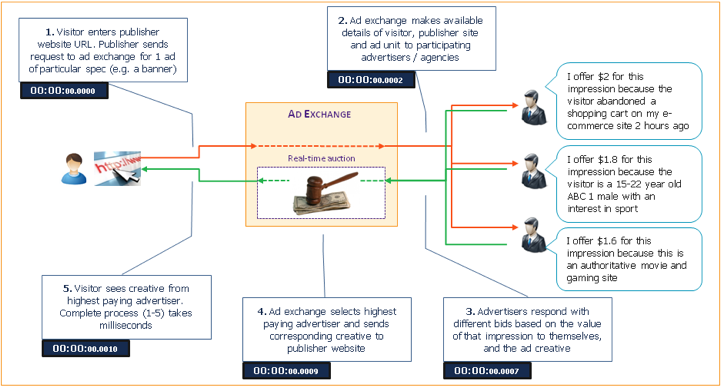
\includegraphics[width=1\textwidth]{adExchange}
    \caption{An example interaction on an Ad Exchange platform \parencite{adExchanges}}
    \label{fig:adExchange}
\end{figure}

\subsection{Targeted Ad Networks}
Targeted Ad networks differ from an Ad network by allowing advertisers to buy audience segments such as: demographics (e.g. gender, age),  behavioural segments (e.g. interest in buying a home), by context (e.g. websites that are in a particular subject area) or by alternatives to Cost Per Mile (CPM) such as cost per 1000 viewers of the advertisement. This holds a significant advantage to advertisers as it offers them the ability to buy on a performance basis. Similarly, this structure offers benefits to publishers who have the ability to sell remnant inventory without without cannibalizing higher priced inventory sold directly / via rep networks \parencite{adExchanges}. Examples of Targeted advertising networks include: Google AdSense, Yahoo! Publisher network, AOL Advertising. 

\subsection{Online Advertising Fraud}
One of the challenges remains in the paradigm of online advertising of how to ensure human users are actually seeing and then clicking through adverts. Bloomberg reported 11\% of display ads and 25\% of video ads displayed on the Internet in 2014 were seen by bots, instead of human users \parencite{bloomFraud}. This correlates with the research of the Financial Times newspaper that found that part of a Mercedes-Benz on-line advertising campaign was viewed more often by computer bots than by human beings. Humans amassing only 43\% of the views \parencite{mercFraud}. Advertising is suffering heavily from the prevelence of Bot Nets, which can be defined as a network of private computers infected with malicious software (malware)  and controlled as a group without the owners' knowledge. In the case of advertising fraud, bot nets are being used when publishers purchase traffic (views) for their website to help boost the price of their advertising inventory. Now publishers are forced to check whether their ads are being viewed or by the ever increasing army of bots. Now that the purchasing of `fake traffic' is so ubiquitous in the advertising industry it has given rise to an industry of countermeasures \parencite{bloomFraud} where publishers are constantly battling the ever increasing number of fake or software related views. A study conducted by the security firm White Ops for the Association of National Advertisers (ANA) concluded that adverts viewed by non-human traffic will cost advertisers \$6.3 billion in 2015. This shows the prevalence and scale of advertising fraud and that advertisers and publishers must work together to help to mitigate the effects of the fake traffic associated with bot nets. Publishers are currently using multiple methods to detect nonhuman traffic however, there is no single standard used by the industry. This form of fraudulent activity is the biggest threat to the online advertising industry. 


\subsection{Tracking}
In terms of this study, tracking will be defined as collecting the personal information and online movements of Internet users for the purpose of using this information to tailor adverts to these users. The most popular method used to collect this data is cookies which are discussed in Section \ref{cookies}. Increasingly advertisers are able to track a user's browsing activities across multiple websites, they can then collate all of this information and use it to better tailor their personalised adverts to an individual user. 

The merits of tracking has been the topic of much debate, as increasingly users feel that their privacy is under threat from intrusive advertisers who collect data in numerous methods. 

\subsection{Tracking Taxonomy}
One of the simplest ways to to classify tracking is based on the domain. There are two different domains for tracking \textit{within site} and \textit{cross site}. Within site tracking is when a first party cookie is used to track a user on the the website that user is viewing. Whereas, cross site tracking refers to tracking the preferences and online movements of Internet users on websites using third-party cookies. A framework has also been suggested by  \parencite{roesner} which classifies web tracking based on the observable behaviours. This framework is shown in Figure \ref{fig:TAframework}. 

\begin{figure}[H]
    \centering
    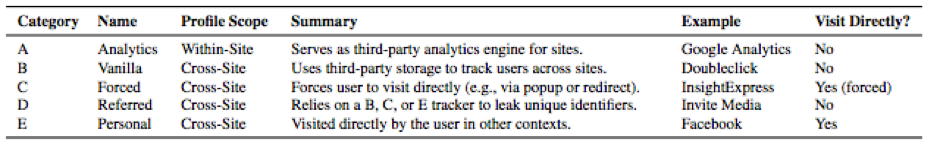
\includegraphics[width=1\textwidth]{TAframework}
    \caption{Framework for classifying web tracking based on observable behaviours \parencite{roesner}}
    \label{fig:TAframework}
\end{figure}

\section{The Arsenal of the Trackers}

\subsection {Cookies} \label{cookies}
A cookie can be defined as a triple (domain,key,value) that is stored in the browser across page visits, where the domain is a particular website and the key and value are opaque identifiers \parencite{roesner}. The cookie mechanism adds state to the otherwise stateless HTTP protocol, as the cookies allow a web server to store a small amount of data on the computers of the visiting users which is then sent back to the web server upon subsequent requests \parencite{cookielessMonster}. There are two types of cookies \textit{first-party} and \textit{third-party}. First-party cookies are set by the domain that the user visits directly, i.e. the domain in the address bar, for example, if a user visits www.google.com then cookies that are set with the domain of www.google.com are first party cookies. Third-party cookies are set by a different domain than the one the user visits, they are embedded in the top-level page, for example if a visitor visits www.amazon.com and the domain of the cookies added are www.google.com then these cookies are third-party cookies. \newline

There are numerous ways cookies can get to a webpage. Traditionally cookies were set by using an HTTP response that included a Set-cookie header, however cookies can appear in a browser in a numerous more subtle methods now. They can be set either by Javascript scripts running in the page or by using an API call from within a plug-in. 

\subsection{Evercookies}
An evercookie is a resilient tracking mechanisms that uses multiple storage vectors including Flash cookies, localStorage, sessionSotage and ETags \parencite{evercookies}. Evercookies use this information to identify a client even after they've removed standard cookies. This is similar to the "respawning" of cookies shown in \parencite{flashCookiesPrivacy} which illustrated the abuse of Flash cookies for regenerating previously removed HTTP cookies. \newline

This abuse of the cookie platform is one of the biggest privacy concern for any Internet user, as these forms of stateful storage actively circumvent user's deliberate attempts to start with a fresh profile. 

\subsection{Cookie Syncing}
Cookie synchronization or cookie syncing is the process of trakcer domains sharing pseudonymous IDs associated with a given user, typically stored in cookies \parencite{webNeverForgets}. This passing of IDs can occur for example when domain A makes a request to a URL hosted by domain B with the pseudonymous ID as parameter within the request. This can be advantageous for organisations as it provides a means for domains to share cookie values and thus the different domains should be able to utilise the information in the cookie to better target adverts to a user's preferences. Observed cookie syncing is indicative of business relationships.  One of the earliest studies of cookie syncing found over 100 syncing events happen on the top 100 Alexa sites \parencite{sellingPrivacy}. A slightly larger scale study was conducted by \parencite{webNeverForgets} and its results can be seen in Figure \ref{fig:cookieSynching}, which were generated from multiple crawls of the top 3,000 Alexa domains. 

\begin{figure}[H]
    \centering
    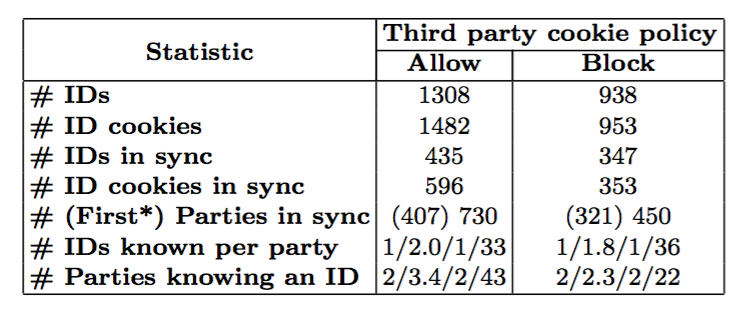
\includegraphics[width=0.75\textwidth]{cookieSynching}
    \caption{Cookie synching statistics from the study of \parencite{webNeverForgets}. The format of the bottom two rows is minimum/mean/median/maximum.}
    \label{fig:cookieSynching}
\end{figure}

These results show that cookie syncing is prevalent upon some of the most visited and trusted sites on the Internet, which would indicate it could ubiquitous across the Internet. The main incentive for trackers to share cookies is the ability to merge databases on the backend based upon the synced IDs. This form of sharing and merging allows trackers to aggregate data in order to obtain a larger fraction of a user's browsing history. As this backend merging occurs behind the closed doors of organisations there is a lack of information of how prevalent the technique is.  However, the financial and mutual benefits for organisations to share tracking information across the ecosystem are significant. As reported by \parencite{webNeverForgets}  101 domains could construct 50\% of a user's browsing history with third-party cookies enabled, this increase in ability to recreate a user's history could have large effects both on user privacy and targeted advertising effectiveness. \newline

The most concerning area of cookie syncing is that it is extremely difficult to block. There are not any tools specifically designed to combat cookie syncing, however a brute force approach would be to block third-party cookie placement and HTTP traffic \parencite{webNeverForgets}, although this lacks practicality. 

\subsection{Fingerprinting}
Another tool available to trackers is device fingerprinting, which aims to identify web users by tracking and collecting their information without the help of cookies. Benign characteristics of a browser's environment like the screen dimensions and list of installed fonts, could be combined to create a unique device-specific finger print analogous to a human biological fingerprint \parencite{uniqueBrowser}. Fingerprinters use attributes that take more diverse values (e.g. the list of fonts) as they are more identifying than values shared by many devices such as user-agent. Furthermore, values which are stable over time facilitate identification compared to those that frequently and unpredictably change \parencite{dustingFP}. 

Again this form of identification of users for tracking purposes is both hard to detect and prevent as the fingerprinting mechanism is not transparent to web users and there are few tools available for users to block it \parencite{uniqueBrowser}. Fingerprinting has been highlighted as an anti-fraud method as it can be used to measure the traffic of a website and prevent click fraud efficiently. However, device fingerprinting allows trackers and advertisers to grab user information despite that users have taken actions to block cookies. This could produce serious privacy concerns for users, as the stateless nature makes it hard to detect, no cookies to inspect and delete, thus even harder to opt-out from. The general unavailability of cookies motivated advertisers and trackers to find new ways of linking users to their browsing histories. All browsers fail to completely hide the user's true identity. 

There are a number of ways to obtain a device fingerprint, this paper will not discuss all of them, it will however detail the most prevalent. A sample of features which can be used to uniquely identify a user can be seen in Figure 4 \ref{fig:fingerprintingConfigs}. Detection of fonts can be one of the most counterintuitively reliable methods to identify a user. Firstly font detection can be carried out by \textit{plugin-based detection} in which \textit{ActionScript} - the scripting language of the Adobe Flash plugin - provides APIs that include methods for discovering the list of fonts installed on a system. Side-channel inference can also be used for font detection, Javascript is used to detect the availability of fonts then deduce the height and width of the fonts comparing this to the predefined standard. Another method frequently used by fingerprinters is two extract information about a user from the browser extensions they have installed. Contemporary browsers are designed in such a way that extensions to the core code base can be added at any time, therefore many people create extensions for browsers to add new functionality or remove undesired functionality. Whilst plugins can be detected via Javascript, extensions cannot be identified by the scripting language, they must be detected by their side effects \parencite{dustingFP}. Paradoxically user-agent spoofing extensions which are meant to hide the identity of a user, were shown by \parencite{cookielessMonster} to actually make a user more identifiable due to inconsistencies in the browsing environment, which in turn made the browsing fingerprint more unique, thus more identifiable. 

\begin{figure}[H]
    \centering
    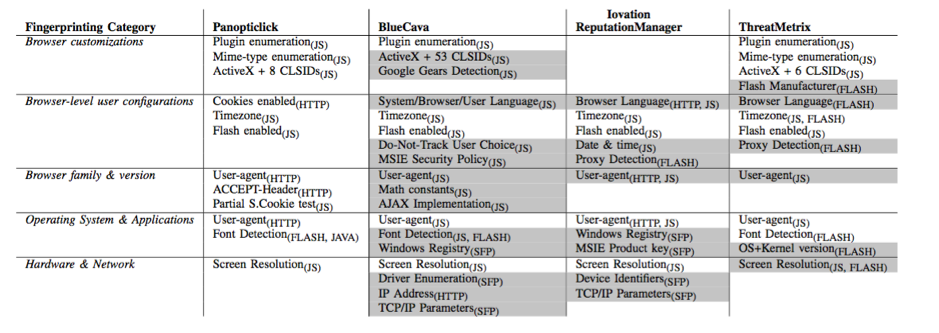
\includegraphics[width=0.75\textwidth]{fingerprintingConfigs}
    \caption{Taxonomy of features used to uniquely fingerprint users \parencite{cookielessMonster}}
    \label{fig:fingerprintingConfigs}
\end{figure}

In an ethical sense fingerprinting can be used constructively or destructively. The line between the constructive and destructive use is, however, largely artificial, because the same technology is used in both cases \parencite{cookielessMonster}. Although it does allow companies to sidestep limitations imposed on tracking by the regulation of cookies in Europe and the USA \parencite{dustingFP}. 

\subsection{Future of Tracking}
Recently announced flash is dead, how will this effect tracking. 

\section{Defences against Tracking}
\subsection{Third Party Cookie Blocking}
Blocking all cookies is uncommon as it could potentially infringe on the functionality of the web, however blocking third party cookies is recommended as the first line of defence against third-party tracking \parencite{roesner}. 


\subsection{Do Not Track}
The Do Not Track (DNT) header is an extension to the HTTP response which allows users to opt out of tracking websites, the extension is accompanied with a wealth of legislation that attempts to give users a standardised way to opt out of web tracking. DNT works by adding an extra HTTP header that is completely compatible with the existing web infrastructure. Whilst this idea is promising in theory a lack of commitment by politicians and enforcement by third party tracking companies has largely resulted in deadlock, as Do Not Track is largely unenforced in the wild. Many papers have cited this lack of enforcement as the main stumbling block for the effectiveness of this process, without a legal or technical requirement the tool will remain largely ineffective. \newline

In contrast with the poor legal and technical support of DNT, people are increasingly worried that this header will create a divided web, as a large amount of free content on the Internet relies upon advertising revenue, there is a worry that people who choose to opt out of tracking by implementing the header may end up not receiving the same content as those who do not. Thus, creating a segregated web, in which the tracking agencies still sit in a position of power. 

\subsection{Disabling Javascript}
In the arsenal of defences against web tracking, the most powerful blunt force weapon a user has is to block the client side scripting language Javascript. This approach is extremely effective at preventing tracking behaviours that require API access to cookies to leak them. Although trackers can still set cookies via HTTP headers, ``Set-Cookie'', and as identified by \parencite{roesner} Behaviour C trackers can use HTML re-directs. Despite this being the most effective single defence available to users disabling Javascript renders much of today's web unusable due to the dynamic nature of web content and reliance upon Javascript. Therefore, making it an impossible solution for many users. 

\medskip
\printbibliography

\end{document}
